
\section{Bow shocks from anisotropic wind--wind interactions}
\label{app:ancantoid}
\begin{figure}
  \centering
  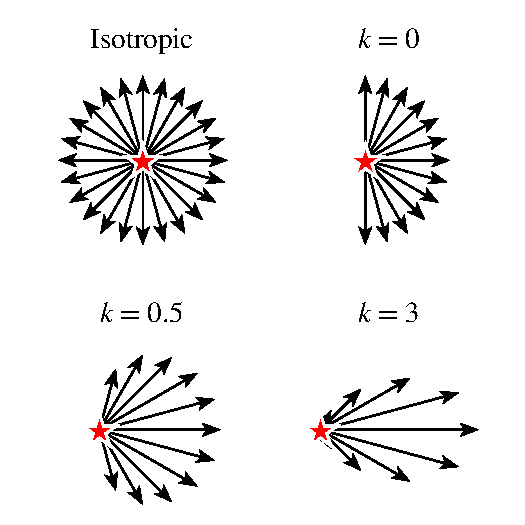
\includegraphics[width=\linewidth]{figs/anisotropic-arrows}
  \caption[]{Schematic diagram of wind flow patterns in isotropic and
    non-isotropic cases for different values of the anisotropy index,
    \(k\).  Arrow length represents the wind momentum loss rate per
    solid angle.}
  \label{fig:anisotropic-arrows}
\end{figure}


We wish to generalize the results of \citet[\CRW{}]{Canto:1996} to the case where the inner wind is no longer isotropic, but instead has a density that falls off with angle away from the symmetry axis.  Specifically, at some fiducial radius, \(r_0\), from the origin, the wind mass density is given by
\begin{equation}
  \label{eq:ancantoid-density}
  \rho(r_0, \theta) =
  \begin{cases}
    \rho_0 \cos^k \theta & \text{for \(\theta \le 90^\circ\)} \\
    0 & \text{for \(\theta > 90^\circ\)}
  \end{cases}
  \ ,
\end{equation}
where \(k \ge 0\) is an anisotropy index.  The wind velocity is still
assumed to be constant and the wind streamlines to be radial, so the
radial variation of density at each angle is
\(\rho(r, \theta) = \rho(r_0, \theta)\, (r/r_0)^{-2}\) and the wind momentum loss rate
per solid angle has the same \(\cos^k\theta\) dependence as the density.


In this work the weakest wind is modeled as an anisotropic hemispherical radial wind
with the following density distribution:
\begin{align}
  n(\theta) = n_0\cos^k\theta
\end{align}  
The index $k$ gives the anisotropy degree. We are interested in winds where $k \geq 0$ for further applications. By the other side, we keep the strongest
wind as isotropic.

The shape of the resultant bow shock is given by:
%If we apply the \CRW{} formalism for a more generalized photoevaporated flow with density given by (\ref{eq:ngen}),
%we find that the solutions for equations (8) - (11) of \CRW{} are the following:

%If we apply the \CRW{} formalism for a generalized photoevaporated flow with density given by equation (\ref{eq:ngen}),
%the shell shape $R(\theta)$ may be calculated from equation (6) of CRW{}:
\begin{align}
  R = \frac{\dot{J}_w + \dot{J}_{w1}}{\left(\dot{\Pi}_{wr}+\dot{\Pi}_{wr1}\right)\cos\theta-\left(\dot{\Pi}_{wz1}+\dot{\Pi}_{wz1}\right)\sin\theta}
  \label{eq:Rmom}
\end{align}

Where:

\begin{align}
\dot{\Pi}_z &= \frac{v_w\dot{M}_w^0}{2(k+2)}\left(1-\cos^{k+2}\theta\right)  \label{eq:pir}\\
\dot{\Pi}_r &= \frac{1}{2}\dot{M}^0_w v_w I_k (\theta) \label{eq:piz}\\
I_k(\theta) & = \int^\theta_0 \cos^k \theta \sin^2\theta~d\theta \label{eq:Ik}\\
\dot{J}_w &= 0 \label{eq:jdot} \\
\dot{M}_w &= \frac{\dot{M}_w^0}{2(k+1)}\left(1-\cos^{k+1}\theta\right) \label{eq:dotprop} \\
M^0_w &\equiv 4\pi v_w r^2_{IF} n_0 \bar{m}\\
\dot{\Pi}_{wz1} & = -\frac{\dot{M}^0_{w1}v_{w1}}{4}\sin^2\theta_1\\
\dot{\Pi}_{wr1} & = \frac{\dot{M}^0_{w1}v_{w1}}{4}\left(\theta_1-\sin\theta_1\cos\theta_1\right)\\
\dot{J}_{w1} & = \frac{\dot{M}^0_{w1}v_{w1}}{4}\left(\theta_1-\sin\theta_1\cos\theta_1\right)D \label{eq:jdot1}
\end{align}

Combining equations  (\ref{eq:pir}) to (\ref{eq:jdot1}) we can obtain numerically the bow shock shape $R(\theta)$ from equation (\ref{eq:Rmom}).
To find the projected shape in the plane of sky, we fit $R(\theta)$ into a quadric curve which has the same characteristic radii $(R_0,R_c,R_{90})$. 
%The most notable scenarios, since they have astrophysical relevance are the following:
%$k=1/2$ ak.a. the ``proplyd case'', following \citep{HA:1998}, and $k=0$, ak.a, the ``isotropic case'', following \CRW{}. The comparison between both solutions
%is shown in figure (\ref{fig:r-beta}), along with an extreme anisotropy case. 

%%% Local Variables:
%%% mode: latex
%%% TeX-master: "quadrics-bowshock"
%%% End:
